% Created 2012-09-26 Wed 23:41
\documentclass[bigger]{beamer}
\usepackage[utf8]{inputenc}
\usepackage[T1]{fontenc}
\usepackage{fixltx2e}
\usepackage{graphicx}
\usepackage{longtable}
\usepackage{float}
\usepackage{wrapfig}
\usepackage{soul}
\usepackage{textcomp}
\usepackage{marvosym}
\usepackage{wasysym}
\usepackage{latexsym}
\usepackage{amssymb}
\usepackage{hyperref}
\tolerance=1000
\usepackage{epigraph}
\mode<beamer>{\usetheme{Boadilla}}
\mode<beamer>{\usecolortheme{crane}}
\mode<beamer>{\useoutertheme[footline=authortitle]{miniframes}}
\institute{The George Washington University}
\providecommand{\alert}[1]{\textbf{#1}}

\title{Pony: Evolving Languages Without (As Many) Bugs}
\author{Andrew Hirsch}
\date{September 27, 2012}

\begin{document}

\maketitle




\begin{frame}
\frametitle{Bugs Are Bad}
\label{sec-1}



\includegraphics{../pictures/no_bug.png}


\begin{itemize}
\item \emph{Bugs} are the errors we find in software
\item Any piece of software probably has many bugs
\item Spoiler: when there are errors in code, things don't work right
\end{itemize}
\end{frame}
\begin{frame}
\frametitle{The Consequences of Bugs}
\label{sec-2}


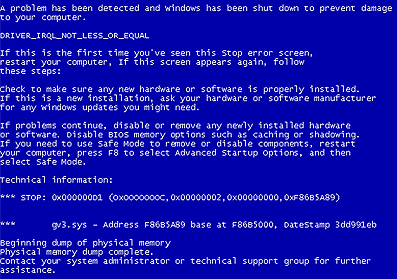
\includegraphics[scale=0.25]{../pictures/BSOD.png}
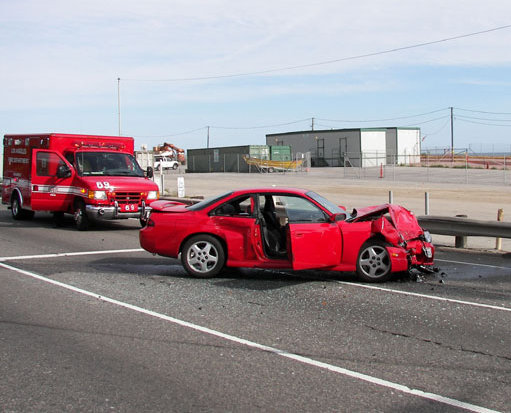
\includegraphics[scale=0.25]{../pictures/car-crash.jpg} \\

\includegraphics[scale=0.25]{../pictures/burning_money.jpg}
\end{frame}
\begin{frame}
\frametitle{The Causes of Bugs}
\label{sec-3}


\epigraph{There are two ways to write error-free programs; only the third one works}{Alan Perlis, "Epigrams on Programming"}


\begin{itemize}
\item What causes bugs?
  \pause
\begin{itemize}
\item Bad Specifications
    \pause
\item Changing Demands
    \pause
\item Multiple Coders
    \pause
\item Poorly Documented Code
    \pause
\item Code ``Too Big To Handle''
\end{itemize}
\end{itemize}
\end{frame}
\begin{frame}
\frametitle{Software is Hard}
\label{sec-4}


\epigraph{Every program attempts to expand until it can read mail. Those programs that cannot so expand are replaced by ones which can.}{Jamie Zawinski}


\begin{itemize}
\item It's nearly impossible to hold all of a (complicated) program in a single head
\item Trying to do so causes lots of bugs
\item How do we fix it?
\end{itemize}
\end{frame}
\begin{frame}
\frametitle{Using Slang}
\label{sec-5}


\epigraph{Slang is a language that rolls up its sleeves, spits on its hands and goes to work.}{Carl Sandburg}


\begin{itemize}
\item We use the phrase ``write code'' for a reason: code is language
\item Slang is often used because it's easier or more expressive
\end{itemize}
\pause

\begin{itemize}
\item Can we add slang to code?
\end{itemize}
\pause

\begin{itemize}
\item Yes!
\item That is the point of Pony
\end{itemize}
\end{frame}
\begin{frame}
\frametitle{Adding Slang to Code}
\label{sec-6}



\includegraphics[scale=0.25]{../pictures/slang.jpg}


\begin{itemize}
\item Since code is a language, let's add slang!
\item First, we make the computer recognize the slang
\item Then, we make it understand the slang
\end{itemize}
\pause

\begin{itemize}
\item But, is this a perfect solution?
\end{itemize}
\end{frame}
\begin{frame}
\frametitle{Problems with Slang}
\label{sec-7}


\epigraph{GIGO:\\ 'Garbage In, Garbage Out'}{The Jargon File}


\begin{itemize}
\item People commonly use different types of slang
\item These different `slangs' might use some of the same words in very different ways
\item How do you tell what they mean?
\end{itemize}
\pause

\begin{itemize}
\item It's easy for a human
\item VERY hard for a computer
\end{itemize}
\pause

\begin{itemize}
\item Pony attempts to tell a programmer when they are in this situation
\end{itemize}
\pause

\begin{itemize}
\item But it's not always possible
\end{itemize}
\end{frame}
\begin{frame}
\frametitle{Conclusion: The Impossible Quest for the Holy Grail}
\label{sec-8}


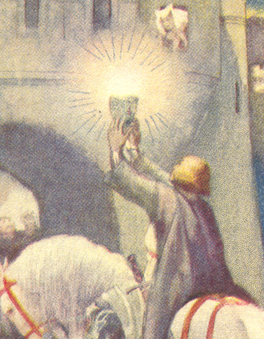
\includegraphics[scale=0.5]{../pictures/holy_grail.jpg}


\begin{itemize}
\item We want to right bug-free code
\item Like the search for the holy grail, it seems impossible
\item However, it is possible to get closer by making it easier for programmers to express themselves
\item Pony is an important step in that process
\end{itemize}
\end{frame}

\end{document}
